\documentclass{article}\usepackage[]{graphicx}\usepackage[]{color}
%% maxwidth is the original width if it is less than linewidth
%% otherwise use linewidth (to make sure the graphics do not exceed the margin)
\makeatletter
\def\maxwidth{ %
  \ifdim\Gin@nat@width>\linewidth
    \linewidth
  \else
    \Gin@nat@width
  \fi
}
\makeatother

\definecolor{fgcolor}{rgb}{0.345, 0.345, 0.345}
\newcommand{\hlnum}[1]{\textcolor[rgb]{0.686,0.059,0.569}{#1}}%
\newcommand{\hlstr}[1]{\textcolor[rgb]{0.192,0.494,0.8}{#1}}%
\newcommand{\hlcom}[1]{\textcolor[rgb]{0.678,0.584,0.686}{\textit{#1}}}%
\newcommand{\hlopt}[1]{\textcolor[rgb]{0,0,0}{#1}}%
\newcommand{\hlstd}[1]{\textcolor[rgb]{0.345,0.345,0.345}{#1}}%
\newcommand{\hlkwa}[1]{\textcolor[rgb]{0.161,0.373,0.58}{\textbf{#1}}}%
\newcommand{\hlkwb}[1]{\textcolor[rgb]{0.69,0.353,0.396}{#1}}%
\newcommand{\hlkwc}[1]{\textcolor[rgb]{0.333,0.667,0.333}{#1}}%
\newcommand{\hlkwd}[1]{\textcolor[rgb]{0.737,0.353,0.396}{\textbf{#1}}}%

\usepackage{framed}
\makeatletter
\newenvironment{kframe}{%
 \def\at@end@of@kframe{}%
 \ifinner\ifhmode%
  \def\at@end@of@kframe{\end{minipage}}%
  \begin{minipage}{\columnwidth}%
 \fi\fi%
 \def\FrameCommand##1{\hskip\@totalleftmargin \hskip-\fboxsep
 \colorbox{shadecolor}{##1}\hskip-\fboxsep
     % There is no \\@totalrightmargin, so:
     \hskip-\linewidth \hskip-\@totalleftmargin \hskip\columnwidth}%
 \MakeFramed {\advance\hsize-\width
   \@totalleftmargin\z@ \linewidth\hsize
   \@setminipage}}%
 {\par\unskip\endMakeFramed%
 \at@end@of@kframe}
\makeatother

\definecolor{shadecolor}{rgb}{.97, .97, .97}
\definecolor{messagecolor}{rgb}{0, 0, 0}
\definecolor{warningcolor}{rgb}{1, 0, 1}
\definecolor{errorcolor}{rgb}{1, 0, 0}
\newenvironment{knitrout}{}{} % an empty environment to be redefined in TeX

\usepackage{alltt}
\usepackage{amscd, amssymb, amsmath, verbatim, setspace}
\usepackage[left=1.0in, right=1.0in, top=1.0in, bottom=1.0in]{geometry}
\usepackage{mathrsfs}
\usepackage{listings}


\IfFileExists{upquote.sty}{\usepackage{upquote}}{}
\begin{document}
\begin{flushright}
  Arif Ali\\
  ANLY-511 HW3\\
  September 30, 2015\\
\end{flushright}
\begin{center}
\end{center}
\section*{Exercise 17}
\begin{knitrout}
\definecolor{shadecolor}{rgb}{1, 1, 1}\color{fgcolor}\begin{kframe}
\begin{verbatim}
X = rbeta(10000, .5, .8)
EX = mean(X)
EX
## [1] 0.3851936
sd(X) #Note: built sd factors in (N-1)/N coeffient
## [1] 0.3224292
sdX = sqrt(mean(X^2)-EX^2)
sdX
## [1] 0.3224131
Ex_.333 = mean(X^(-1/3))
Ex_.333
## [1] 2.707823
\end{verbatim}
\end{kframe}
\end{knitrout}
\section*{Exercise 18}
\begin{knitrout}
\definecolor{shadecolor}{rgb}{1, 1, 1}\color{fgcolor}\begin{kframe}
\begin{verbatim}
EsqrtX = replicate(1000, mean(sqrt(rbeta(10000, .5, .8))))
mean((EsqrtX))
## [1] 0.5436174
sd(EsqrtX)
## [1] 0.003125486
rep(mean((EsqrtX)), times = 2) + 4*c(-sd(EsqrtX), sd(EsqrtX))
## [1] 0.5311155 0.5561194
\end{verbatim}
\end{kframe}
\end{knitrout}
Based on the following simulation, the range in which $E(\sqrt{X})$ is between 0.5316151 and 0.5558636. The endpoints range were
determined by looking at the values that were 4 standard deviations ($\frac{N-1}{N}$ correction from R) from the mean. Thus, the
approximate of $E(\sqrt{X})$ has a confidence interval of greater than 99.9 percent.  
\section*{Exercise 19}
\begin{knitrout}
\definecolor{shadecolor}{rgb}{1, 1, 1}\color{fgcolor}\begin{kframe}
\begin{verbatim}
X = runif(25000)
Y = runif(25000)
Z = X[Y<=(sin(2*pi*X))^2]
hist(Z)
\end{verbatim}
\end{kframe}
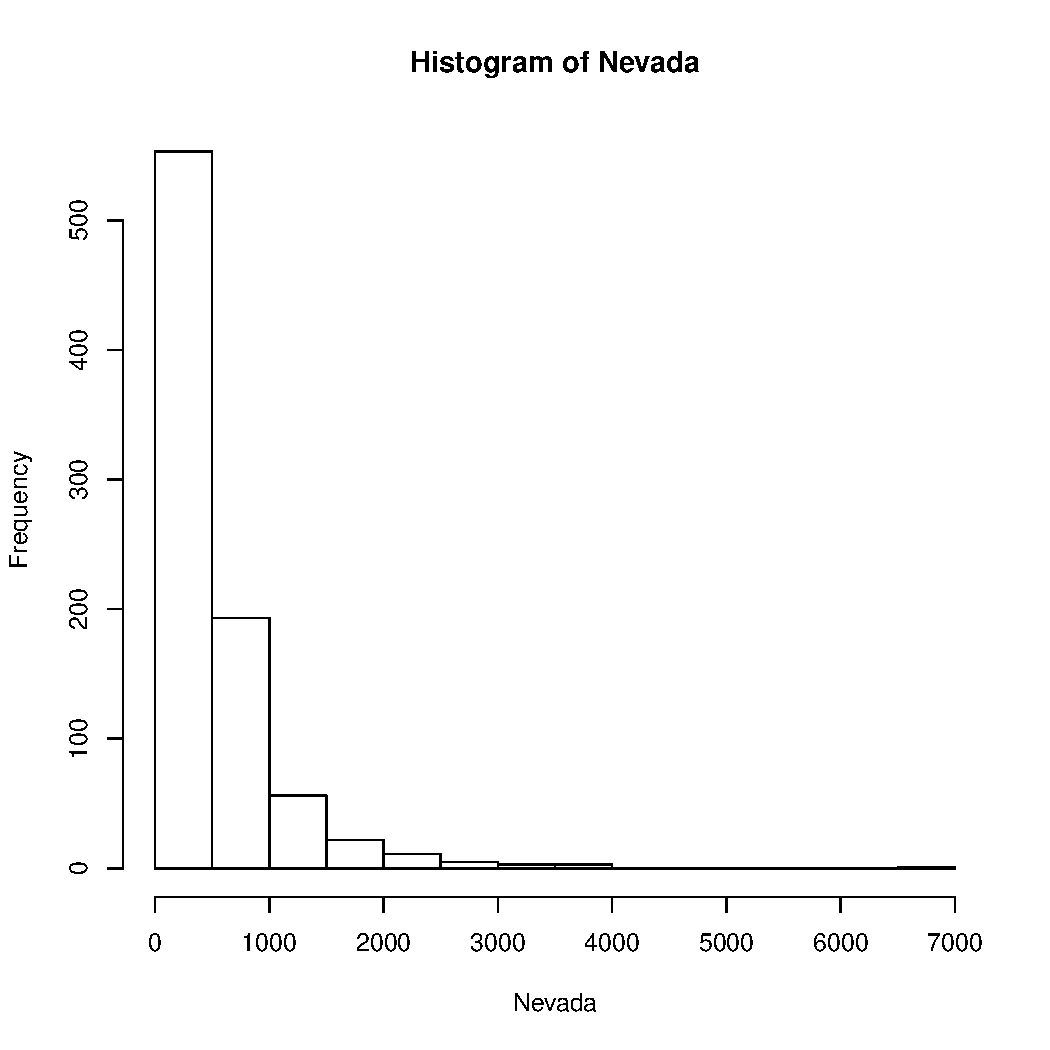
\includegraphics[width=0.33\linewidth]{figure/unnamed-chunk-4-1} 

\end{knitrout}
The histogram of Z takes on a shape that have to peaks. It looks like two normal distribution histograms side by side. The peaks on both of these normal distribtuion like instances look to be approximately the same
\section*{Exercise 20}
\subsection*{a}
\begin{knitrout}
\definecolor{shadecolor}{rgb}{1, 1, 1}\color{fgcolor}\begin{kframe}
\begin{verbatim}
sensitivity = 0.99/(0.99+0.01)
sensitivity
## [1] 0.99
specificity = 0.99/(0.99+0.02)
specificity
## [1] 0.980198
\end{verbatim}
\end{kframe}
\end{knitrout}
\subsection*{b}

\begin{knitrout}
\definecolor{shadecolor}{rgb}{1, 1, 1}\color{fgcolor}\begin{kframe}
\begin{verbatim}
(0.99/500)/((0.99/500)+0.02*499/500)
## [1] 0.09024613
\end{verbatim}
\end{kframe}
\end{knitrout}
\section*{Exercise 21}
Please see next page.
\section*{Exercise 22}
\begin{knitrout}
\definecolor{shadecolor}{rgb}{1, 1, 1}\color{fgcolor}\begin{kframe}
\begin{verbatim}
aBunchOfCauchyDistributions = replicate(1000, rcauchy(1000))

meanOfABunchOfCauchyDistributions = rowSums(aBunchOfCauchyDistributions)/1000

par(mfrow=c(3, 2))

Fx = pcauchy(meanOfABunchOfCauchyDistributions)
plot(ecdf(Fx), main = "Mean where N = 1000")

for(i in sample(1:1000, 5)){
Fx = pcauchy(aBunchOfCauchyDistributions[,i])
plot(ecdf(Fx), main = c("Cauchy column:",i)) 
}
\end{verbatim}
\end{kframe}
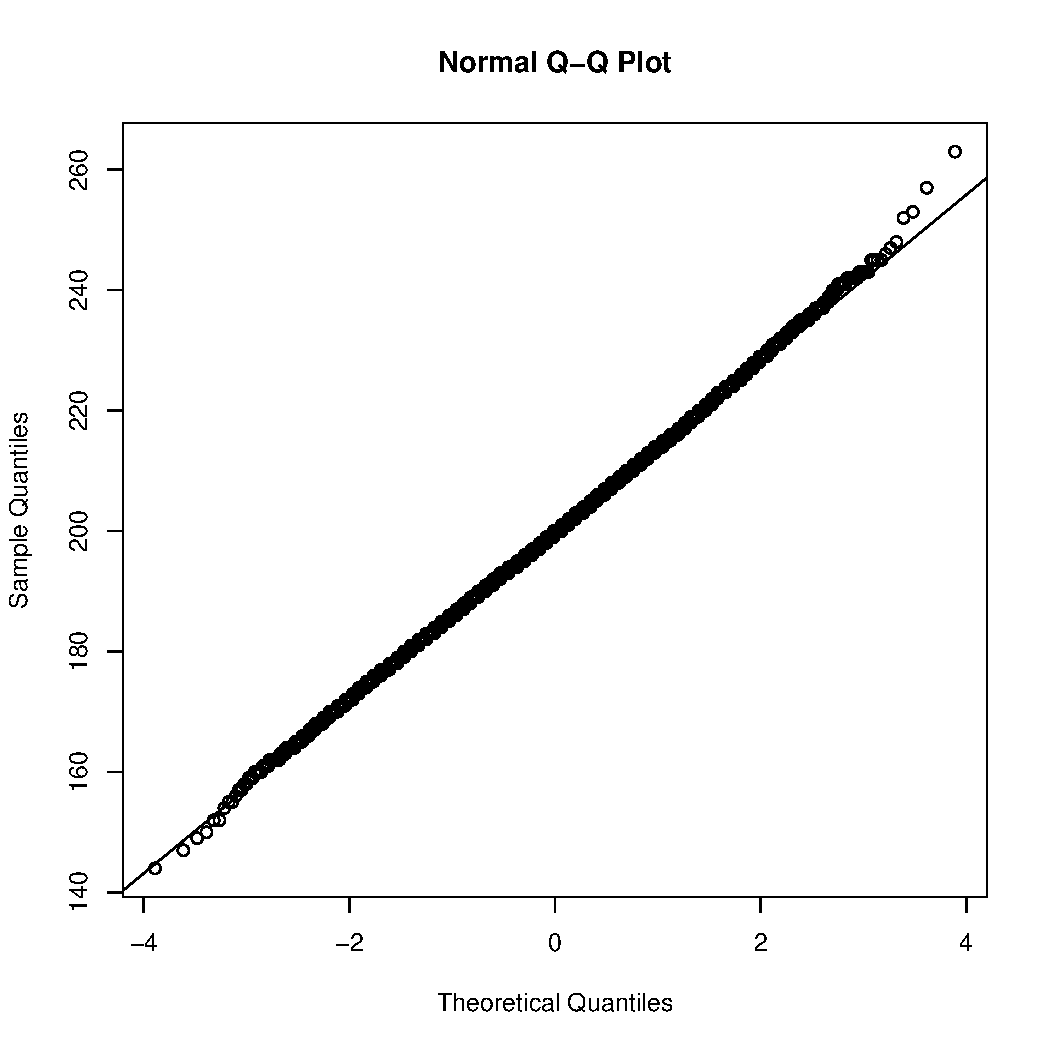
\includegraphics[width=0.33\linewidth]{figure/unnamed-chunk-7-1} 
\begin{kframe}\begin{verbatim}
aBunchOfCauchyDistributions = replicate(500, rcauchy(1000))

meanOfABunchOfCauchyDistributions = rowSums(aBunchOfCauchyDistributions)/500

par(mfrow=c(3, 2))

Fx = pcauchy(meanOfABunchOfCauchyDistributions)
plot(ecdf(Fx), main = "Mean where N = 500")

for(i in sample(1:500, 5)){
Fx = pcauchy(aBunchOfCauchyDistributions[,i])
plot(ecdf(Fx), main = c("Cauchy column:",i)) 
}
\end{verbatim}
\end{kframe}
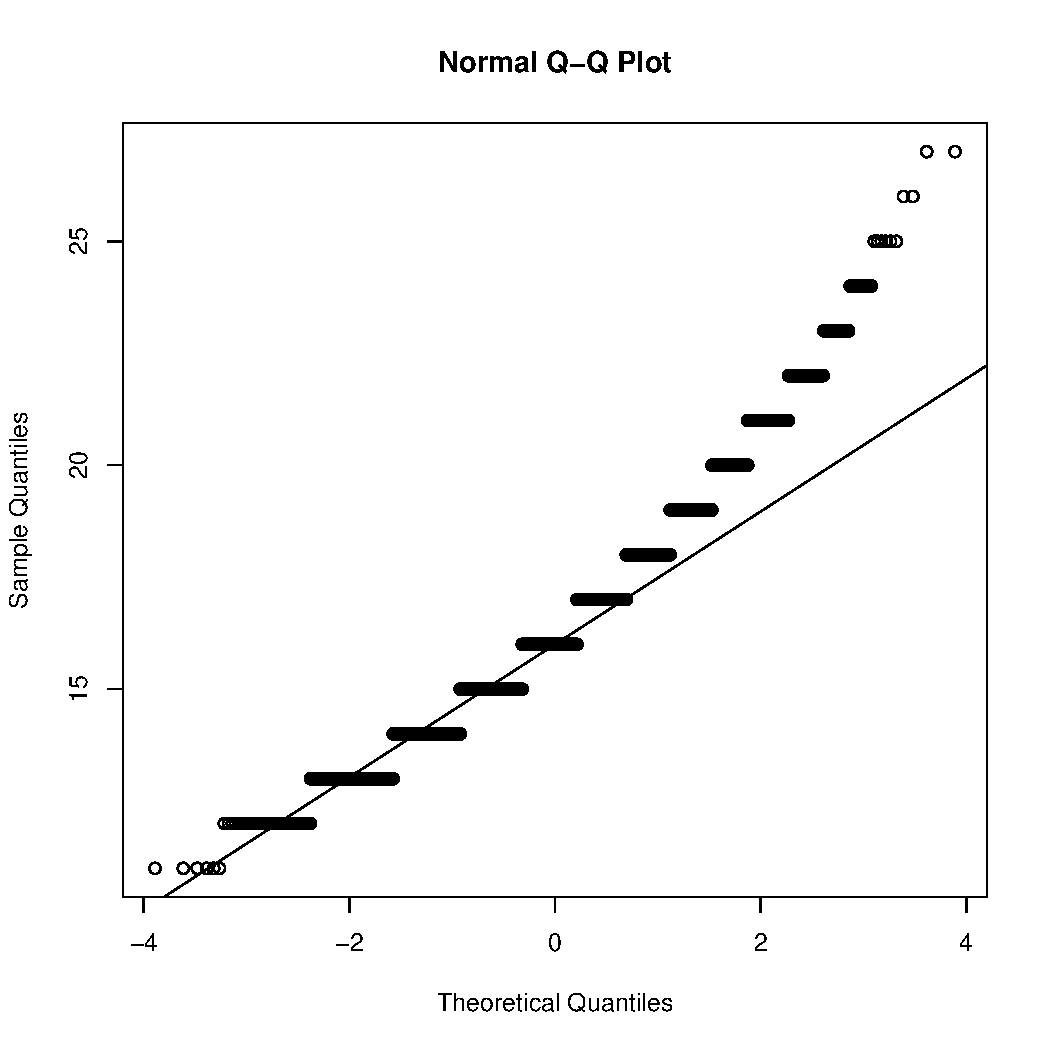
\includegraphics[width=0.33\linewidth]{figure/unnamed-chunk-7-2} 

\end{knitrout}
Following the same method used in the previous homework with respect to the similarities of exponential distributions with respect to uniform distributions. I used the same method (ecdf) to compare the mean of N cauchy distributions (N being either 1000 or 500) and please note how the graph of the means are near identical to 5 different cauchy distributions. they are a straight line over the same x values.


Please see next page for the remaining problems (21,23, and 24)
\end{document}
